\documentclass[14pt, a4paper]{article}
\usepackage{amsmath}
\usepackage{amssymb}
\usepackage[style=authoryear, backend=biber, maxnames=3]{biblatex} % for the citation, 
\usepackage{hyperref}
\addbibresource{bibentries.bib}
\usepackage{graphicx}
\usepackage[utf8]{inputenc}
\setlength\parindent{0pt}
\renewcommand{\baselinestretch}{1.5} 
\graphicspath{{../../}}



\title{Sophia's \& Marcel's Stat Bible:\\ A collaborative collection of useful shit}
\author{Sophia Gläser\thanks{Zeppelin Universität}\ and 
Marcel Schliebs\footnotemark[2]\
 \thanks{Correspondence should be addressed to Marcel Schliebs, Zeppelin Universität, Am Seemooser Horn 20 in D-88045 Friedrichshafen, Germany. E-mail: m.schliebs@zeppelin-university.net}}
\date{A first beta version (\textit{Version as of \today})}

\begin{document}
\maketitle

\rule{\linewidth}{0.4pt}
\begin{abstract}
This is the abstract
\end{abstract}
\textbf{Keywords:} asdasd, asd, asd\\
\medskip
\textbf{JEL codes:} asdasd, asd, asd\\
\rule{\linewidth}{0.4pt}


\maketitle

\tableofcontents
\newpage


\section{Mathematical Basics}

...\\
...\\
...\\
...\\
...\\
...\\

\section{Introductory Statistics}

\subsection{Descriptive Statistics}

\subsection{Jan zahlt mir heute Höpker}

\subsection{Statistical Inference}

\section{Advanced Econometrics}

\subsection{Multivariate linear Regression}

\subsection{Time Series Analysis}


\section{Data Analysis Using R}
\subsection{R Basics}
\subsection{Data Management}
\subsection{Data Visualization}


\section{Bayesian Data Analysis}


\section{Quantitative Finance}


\section{Next steps}







\begin{figure}
\caption{A Figure using R}
\centering
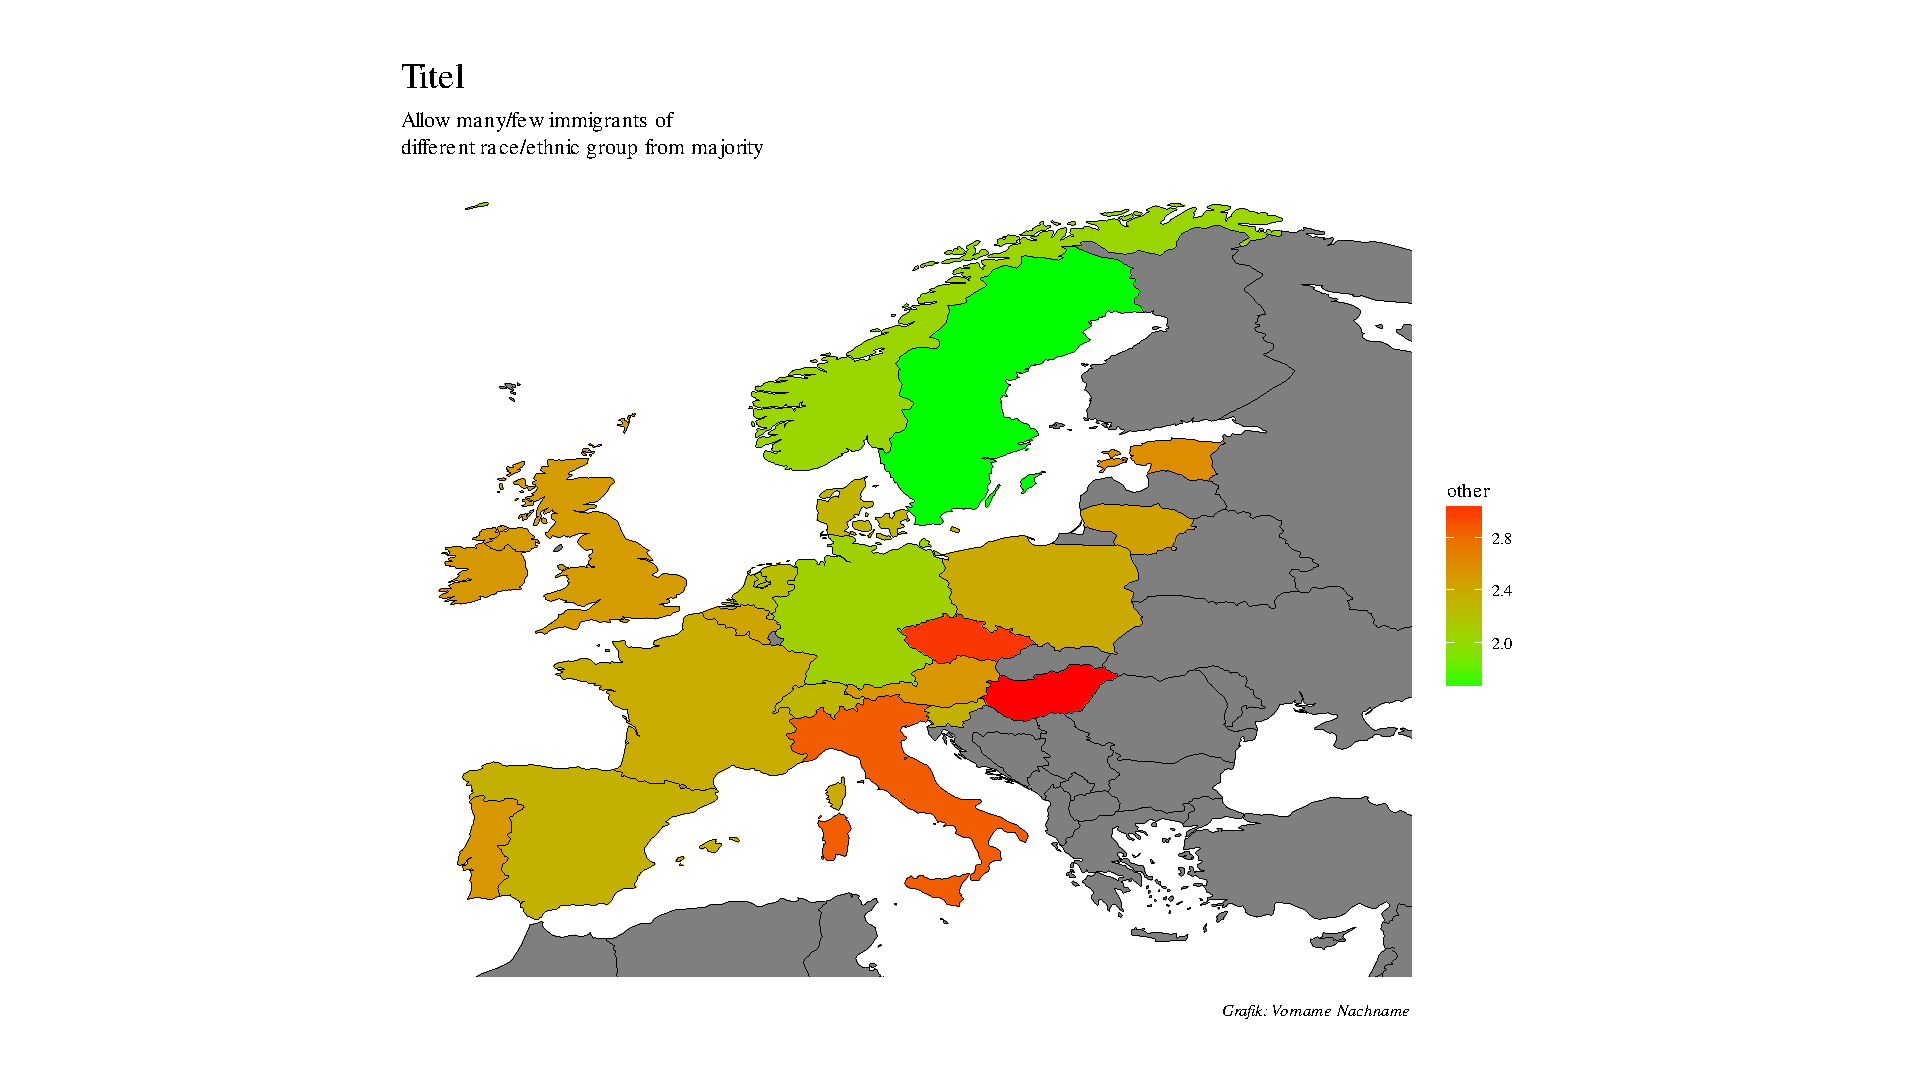
\includegraphics[width=0.75\textwidth]{results/figures/a3.pdf}
\end{figure}



\begin{table}
\begin{scriptsize}
%\input{tables/table1}
\end{scriptsize}
\caption{A table using stargazer}
\end{table}

\begin{table}
\begin{scriptsize}
%\input{tables/table2}
\end{scriptsize}
\caption{Another table using stargazer}
\end{table}

\newpage

\printbibliography
\end{document}